\chapter{Elementary Notions about Graphs}

\begin{descr}
\end{descr}

\section{Undirected Graphs}
\begin{definition}
	An undirected graph is a pair G=(V, E) where V is a set of nodes and E is a set of edges, together with a function i: E $\rightarrow \gamma(v)$ such that 0 < $\mid i(e) \mid  \le $ 2.
\\
If u,v i(e) we call u,v endpoints of e. \\
If V and E are a finite set we call G a finite graph. \\
If i($e{_1}$) =  i($e{_2}$) we call  $e{_1}$, $e{_2}$ parallel edges.\\
If $\mid i(e) \mid = 1$ we call e a loop. \\
The degree of a node v is the number of edges for which v is an endpoint where loops a counted twice.\\
Is the degree of v = 0 then we call v isolated.
\end{definition}

\begin{example*}
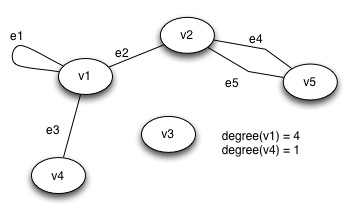
\includegraphics{diagrams/Chapter1_Example1.jpg} \\
\end{example*}

\begin{lemma}
    In a finite graph the number of nodes with odd degree is even.
\end{lemma}


\begin{prooof}
    $\sum\limits_{i=1}^n degree(v_{i}) = 2* \mid E \mid$ \\
This is because we start with a graph, where each node is isolated. Then we insert one edge after another.\\
Case 1: i(e) = {x} then the degree of x is increased by 2\\
Case 2: i(e) = {x, y} then the degree of x and y are increased by 1\\
We asume that $v_{1}...v_{i}$ have an even degree and $v_{i+1}...v_{n}$ have odd degree.\\

$\sum\limits_{k=1}^i degree(v{_k}) + \sum\limits_{k=i+1}^n degree(v{_k}) = 2 \mid E \mid$\\

$\sum\limits_{k=1}^i degree(v{_k})$ is an even number\\

$\sum\limits_{k=i+1}^n degree(v{_k})$ must be an even number and hence the number of nodes with odd degree must be even\\

$ 2 \mid E \mid$ is an even number \\

\end{prooof}


\begin{definition}
    If G=(V,E) is a graph and $v{_1}, v{_2} \in V$ with $i(e) = \{v_1, v_2\}$ then we say that $v{_1}, v{_2}$ are neighbours. \\
    A path in G is a sequence of edges $e{_1}, e{_2}, ...$ such that: \\
\begin{enumerate}
\item $e{_i}, e_{i+1}$ share an endpoint
\item if $e{_i}$ is not a loop and neither the first nor the last edge. Then $e{_i}$ shares one endpoint with $e_{i-1}$ and the other with $e_{i+1}$ [MS: does this make sense? sounds strange!][NW: Yes, draw it]
\end{enumerate}
\end{definition}

\begin{example*}
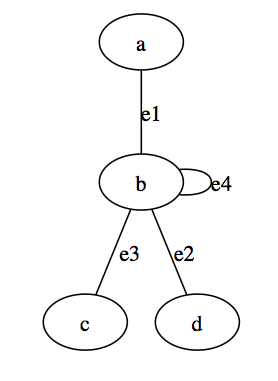
\includegraphics[scale=0.5]{diagrams/Chapter1_Example2}
\end{example*}

A finite graph is graphically represented by: $v{_0}$ --- $v{_1}$ --- $v{_2}$ --- ... --- $v{_i}$\\
$v{_0}$ is called start point and $v{_i}$ is called end point. The length of the path $e{_1}$ ... $e{_i}$  is $i$.\\
\\
A cycle (circle) is a path where the end point coincide with the start point.\\
A path is called simple if every node in $V$ occures at most once.\\
A cycle of length $\neq 2$ is called simple if every node except of the start/end node occurs at most once. \\
A cycle of length 2 ($e{_1}$, $e{_2}$) is called simple if $e{_1} \neq e{_2}$ and if each node except for the start/end node occurs at most once.

\begin{example*}
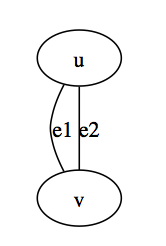
\includegraphics[scale=0.4]{diagrams/Chapter1_Example3}
Simple\\
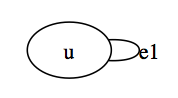
\includegraphics[scale=0.4]{diagrams/Chapter1_Example4}
Simple\\
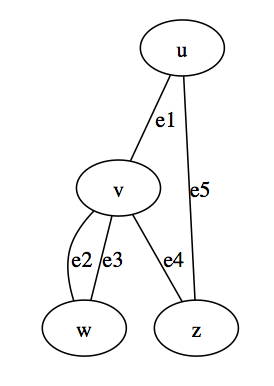
\includegraphics[scale=0.45]{diagrams/Chapter1_Example5}
Not simple\\
\end{example*}

A Graph is connected if for every pair of nodes ($u$, $v$) there is a path between $u$ and $v$.\\

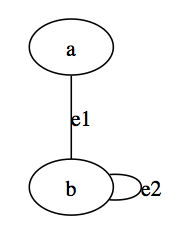
\includegraphics[scale=0.45]{diagrams/Chapter1_Example6}

An infinite Graph has finite and infinite paths. Every path between two nodes is finite. The graph is connected. There are infinitely paths.\\
e.G. $e{_1}$ (finite)\\
or $e{_1}$, $e{_2}$\\
...\\
and there is also an infite path $e{_1}$, $e{_2}$, $e{_2}$, $e{_2}$, $e{_2}$, $e{_2}$, ...\\


\begin{definition}
    Let $G(V,E)$ be a connected graph $a \in V$ is called a seperation point (articulation point) if there are nodes $v, w$ such that every path connecting $v$ and $w$ visits $a$. If $G$ has such a point $G$ is called [word missing - MS]\\
    An edge is called bridge if there exist nodes $v$, $w$ such that every path connecting $v$ and $w$ contains this edge.
\end{definition}

\begin{example*}
Real-Life examples where seperation points are important are in computer networks or the information distribution (flow of information) within a company. So a seperation point can be regarded as a kind of coordinator between $a$ and $b$.
\end{example*}

\begin{definition}
    Let $G = (V,E)$ be a graph without loops. If there exists $V_{1}, V_{2} \subseteq V$ and $V_{1} \cup V_{2} = V$
    such that $V_{1} \cap V_{2} = \emptyset$ and every edge $e$ has one endpoint in $V{_1}$ and the other in $V_{2}$,
    then we call $G$ a \deftxt{bipartite}.
\end{definition}

\begin{example*}
    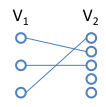
\includegraphics{diagrams/def14_example1.png}
\end{example*}

\begin{definition}
    A directed graph is a pair $G = (V,E)$ where $V$ is a set of nodes (vertices) and $E$ is a set of edges together 
    with a function $i: E -> V x V$. If $i(e) = (v_{1},v_{2})$ then $v_{1}$ is called start point, $v_{2}$ is called end point.
\end{definition}
Graphically: \\[3mm]
If $i(e) = (v_{1},v_{2})$ we draw 1. \\
If $i(e') = (v_{1},v_{2})$ then this indices a second edge (2.). \\
If $i(e_{1}) = i(e_{2})$ we call $e_{1},e_{2}$ parallel. \\
If $i(e) = (v,v)$ then $e$ is called a directed loop. \\
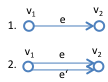
\includegraphics{diagrams/def15_directd_graph.png} \\
$g_{out}(v)$ is the number of edges that have starting point $v$. \\
$g_{in}(v)$ is the number of edges with endpoint $v$.

\begin{lemma}
    $\displaystyle\sum\limits_{v \in V} g_{in}(v) = \displaystyle\sum\limits_{v \in V} g_{out}(v)$
\end{lemma}

\begin{prooof}
    We start with a graph without edges. Then we insert one after the other edges in $E$. 
    Each edge contributes 1 to both sides of the equation.
\end{prooof}

\section{Directed Graphs}
\begin{definition}
    A directed path is a sequence of edges $e_{1},e_{2}...$ such that the end point of $e_{i}$ is the start point of
    $e_{i+1}$\\[3mm]

    A directed path $e_{1}...e_{k}$ is called a (directed) \underline{cycle}, if the start point of $e_{1}$ and
    the end point of $e_{k}$ coincide. \\
    A simple (directed) path is a path where every node occurs at most once. \\
    A directed cycle is called simple if every node except for the start and end node occurs at most once.
\end{definition}

\begin{definition}
    A graph directed or undirected is called \underline{simple}, if it does not contain parallel edges.
\end{definition}

\begin{definition}
        A directed graph is called \underline{strongly connected} if for any pair of nodes $(u,v)$ 
        there is a directd path from $u$ to $v$.
\end{definition}

Let $G$ be a directed graph $G = (V,E)$. $x,y \in V x \textasciitilde y$ ([NW] does \textasciitilde mean are "connected"?)
if there is a directed path from x to y and vice versa. \\

The equivalence classes of this relation $~c VxV$ are called strongly connected components.
(Analogously: Define connected components for undirected graphs)

\begin{information}
    We should know how the following terms are defined: reflexivity, symetry, transitivity.
\end{information}

\section{Implementation of Graphs on Computers}
1. Adjacency Lists $V = {1...n}, E = {e_{1}...e_{t}}$ \\
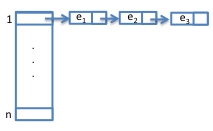
\includegraphics{diagrams/adjacency_list.png} \\
2. Dynamically changing graphs: \\
e.g. multi user databses: Nodes $\equiv$  transactions of user; Edges $\equiv$  waiting situations \\
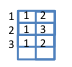
\includegraphics{diagrams/dynamically_changing_graphs.png} \\
Graph is used to detect dead locks. Waiting arises when data are locked by a user that modifies these data. \\
$U_{1}$ $write(d)$, $read(d')$ \\
$U_{2}$ $read(d)$, $write(d')$

\section{Trees}
\begin{definition}
    An undirected graph is called a tree if it is connected and does not have simple cycles.\\
    Let $G$ be a directed graph, $G=(V,E)$. A node $r$ is called root if every other node can be 
    reached from $r$ via a directed path. \\
    A directed graph is called a tree if it has a root and the underlying undirected graph is a tree. \\
    Let $G$ be a directed graph. A node is called source if $g_{in}(v) = 0$. $v$ is called sink if $g_{out}(v) = 0$
\end{definition}

\begin{lemma}
    NW: what was lemma 1.3? the next one was 1.4 in my notes
\end{lemma}
\begin{lemma}
    If $G=(V,E)$ is a directed graph without directed cycles, then there is always a source and sink.
\end{lemma}
We use this theorem to detect cycles

\begin{prooof}[Proof: Source (sink analogously)]
    Select an arbitrary node $v_{1}$. If $v_{1}$ is a source we are done. If it is not, then there must be an edge $e_{1}$
    leading to it $v_{2} \xrightarrow{e_{1}} v_{1}$. \\
    If $v_{2}$ is a source we are done. If not, there must be an edge $e_{2}$ leading to it
    $v_{3}  \xrightarrow{e_{2}} v_{2} \xrightarrow{e_{1}} v_{1}$.
    We continue this process. It must stop because there are only finitely many nodes and if a node would appear once more
    on such a path, there would be a directed cycle.
\end{prooof}






